% The generic preamble
\documentclass[10pt,letterpaper,fleqn,titlepage]{article}

% Define packages to use
\usepackage{natbib}
\usepackage[dvips]{graphicx,color}
\usepackage{amsmath,amssymb}
\usepackage{bm}
\usepackage{caption}
\usepackage{xr}
\usepackage{ifthen}
\usepackage[dvipdfm,colorlinks,linkcolor=blue,citecolor=blue,urlcolor=blue]{hyperref}
\usepackage{fancybox}
\usepackage{textcomp}
\usepackage{alltt}
%\usepackage{floatflt}
%\usepackage{svn}


% Redefine default page
\setlength{\textheight}{9in}  % 1" above and below
\setlength{\textwidth}{6.75in}   % 0.5" left and right
\setlength{\oddsidemargin}{-0.25in}

% Redefine default paragraph
\setlength{\parindent}{0pt}
\setlength{\parskip}{1ex plus 0.5ex minus 0.2ex}

% Define caption width and default fonts
\setlength{\captionmargin}{0.5in}
\renewcommand{\captionfont}{\sffamily}
\renewcommand{\captionlabelfont}{\bfseries\sffamily}

% Define commands for super- and subscript in text mode
\newcommand{\superscript}[1]{\ensuremath{^\textrm{#1}}}
\newcommand{\subscript}[1]{\ensuremath{_\textrm{#1}}}

% Derived commands
\newcommand{\invcm}{\textrm{cm\superscript{-1}}}
\newcommand{\micron}{\ensuremath{\mu\textrm{m}}}

\newcommand{\df}{\ensuremath{\delta f}}
\newcommand{\Df}{\ensuremath{\Delta f}}
\newcommand{\dx}{\ensuremath{\delta x}}
\newcommand{\Dx}{\ensuremath{X_{max}}}
\newcommand{\Xeff}{\ensuremath{X_{eff}}}

\newcommand{\water}{\textrm{H\subscript{2}O}}
\newcommand{\carbondioxide}{\textrm{CO\subscript{2}}}
\newcommand{\ozone}{\textrm{O\subscript{3}}}

\newcommand{\taup}[1]{\ensuremath{\tau_{#1}}}
\newcommand{\efftaup}[1]{\ensuremath{\tau_{#1}^{*}}}

\newcommand{\textbfm}[1]{\boldmath\ensuremath{#1}\unboldmath}

\newcommand{\rb}[1]{\raisebox{1.5ex}[0pt]{#1}}

\newcommand{\f}[1]{\texttt{#1}}

% Define how equations are numbered
\numberwithin{equation}{section}
\numberwithin{figure}{section}
\numberwithin{table}{section}

% Define a command for title page author email footnote
\newcommand{\email}[1]
{%
  \renewcommand{\thefootnote}{\alph{footnote}}%
  \footnote{#1}
  \renewcommand{\thefootnote}{\arabic{footnote}}
}

% Define a command to print the Office Note subheading
\newcommand{\notesubheading}[1]
{%
  \ifthenelse{\equal{#1}{}}{}
  { {\Large\bfseries Office Note #1\par}%
    {\scriptsize \sc This is an unreviewed manuscript, primarily intended for informal}\\ 
    {\scriptsize \sc exchange of information among JCSDA researchers\par}%
  }
}

% Redefine the maketitle macro
\makeatletter
\def\docseries#1{\def\@docseries{#1}}
\def\docnumber#1{\def\@docnumber{#1}}
\renewcommand{\maketitle}
{%
  \thispagestyle{empty}
  \vspace*{1in}
  \begin{center}%
     \sffamily
     {\huge\bfseries Joint Center for Satellite Data Assimilation\par}%
     \notesubheading{\@docnumber}
  \end{center}
  \begin{flushleft}%
     \sffamily
     \vspace*{0.5in}
     {\Large\bfseries\ifthenelse{\equal{\@docseries}{}}{}{\@docseries: }\@title\par}%
     \medskip
     {\large\@author\par}%
     \medskip
     {\large\@date\par}%
     \bigskip\hrule\vspace*{2pc}%
  \end{flushleft}%
  \newpage
  \setcounter{footnote}{0}
}
\makeatother
\docseries{}
\docnumber{}


% Define a command for a DRAFT watermark
\usepackage{eso-pic}
\newcommand{\draftwatermark}
{
  \AddToShipoutPicture{%
    \definecolor{lightgray}{gray}{.85}
    \setlength{\unitlength}{1in}
    \put(2.5,3.5){%
      \rotatebox{45}{%
        \resizebox{4in}{1in}{%
          \textsf{\textcolor{lightgray}{DRAFT}}
        }
      }
    }
  }
}




\includeonly{sndr_g14.app,sndr_g15.app}

% Subversion keywords
\SVN $Date$
\SVN $Revision$

% Title info
\title{GOES-14 and -15 Sounder Spectral Response Functions}
\author{Paul van Delst\email{paul.vandelst@noaa.gov}\\JCSDA/EMC/SAIC\\[0.25in]
        David Groff\email{david.groff@noaa.gov}\\JCSDA/EMC/SAIC}
\date{\SVNDate ; rev\SVNRevision}
\docnumber{ }
\docseries{CRTM}


%-------------------------------------------------------------------------------
%                            Ze document begins...
%-------------------------------------------------------------------------------
\begin{document}
\maketitle

%\draftwatermark

\setcounter{page}{1}

\section{Introduction}
%=====================
This document examines the spectral response functions (SRFs) of the GOES-O(14) and -P(15) sounder instrument. These SRFs are used to generate instrument resolution transmittances and, from those, transmittance model coefficients for use in the CRTM.

The original SRF data was obtained from the \href{http://cimss.ssec.wisc.edu/goes/calibration/SRF}{CIMSS GOES Calibration website} in September 2008 and some anomalous features were identified. Revised SRF data from ITT was received in April 2010 (GOES-14) and June 2010 (GOES-15). This document has been updated to determine if the anomalies in the original SRF data have been removed.


\clearpage
\section{GOES-O(14) Sounder SRFs}
%================================

\subsection{Nominal SRF plots}
%-----------------------------
Plots of the revised SRF data for each channel detector, along with the detector average, are shown in appendix \ref{app:sndr_g14}. SRF plots for channels 1-6 are shown in figure \ref{fig:sndr_g14.ch1-6}, channels 7-12 in figure \ref{fig:sndr_g14.ch7-12}, and channels 13-18 in figure \ref{fig:sndr_g14.ch13-18}.


\subsection{Old Anomalous Features}
%----------------------------------
Inspection of the original GOES-0(14) sounder SRFs showed both ambiguous and clear anomalies for several channels. Comparisons of the original and revised SRF data for the suspect channels are shown in figures \ref{fig:sndr_g14.ch5.anomaly} to \ref{fig:sndr_g14.ch12.anomaly}.

\subsubsection{Channel 5}
%........................
\begin{description}
  \item[Original SRF:] The begin point of this channel was unlike any others in that it starts at a relatively large value.
  \item[Revised SRF:]  The anomaly is no longer present. See figure \ref{fig:sndr_g14.ch5.anomaly}.
\end{description}

\begin{figure}[htp]
  \centering
  \begin{tabular}{c c}
    \multicolumn{2}{c}{\textsf{\bfseries High begin point value}} \\
    \hspace{2.0em}\textsf{Original Data} &
    \hspace{2.0em}\textsf{Revised Data} \\
    \includegraphics[scale=0.5,trim=0 40 0 0]{graphics/zoom_anomaly/original/sndr_g14.ch5.srf.eps} &
    \includegraphics[scale=0.5,trim=0 40 0 0]{graphics/zoom_anomaly/revised/sndr_g14.ch5.srf.eps} \\\\
  \end{tabular}
  \caption{Magnification of GOES-O(14) Sounder individual detector and average SRFs for channel 5. The detector average SRF is plotted in black. \textbf{(Left Panel)} Original SRF data showing the anomaly. \textbf{(Right Panel)} Revised SRF data with no anomaly.}
  \label{fig:sndr_g14.ch5.anomaly}
\end{figure}

\subsubsection{Channel 6}
%........................
\begin{description}
  \item[Original SRF:] The negative values for the low-frequency beginning portions of this SRF have been truncated. The shape of the remaining positive data begged the question: are these data real or an artifact of the fitting algorithm (high order polynomial or spline)?
  \item[Revised SRF:]  The anomaly is no longer present. See figure \ref{fig:sndr_g14.ch6.anomaly}.
\end{description}

\begin{figure}[htp]
  \centering
  \begin{tabular}{c c}
    \multicolumn{2}{c}{\textsf{\bfseries Negative truncation. Are positive values a fit artifact?}} \\
    \hspace{2.0em}\textsf{Original Data} &
    \hspace{2.0em}\textsf{Revised Data} \\
    \includegraphics[scale=0.5,trim=0 40 0 0]{graphics/zoom_anomaly/original/sndr_g14.ch6.srf.eps} &
    \includegraphics[scale=0.5,trim=0 40 0 0]{graphics/zoom_anomaly/revised/sndr_g14.ch6.srf.eps} \\\\
  \end{tabular}
  \caption{Magnification of GOES-O(14) Sounder individual detector and average SRFs for channel 6. The detector average SRF is plotted in black. \textbf{(Left Panel)} Original SRF data showing the anomaly. \textbf{(Right Panel)} Revised SRF data with no anomaly.}
  \label{fig:sndr_g14.ch6.anomaly}
\end{figure}

\subsubsection{Channel 9}
%........................
\begin{description}
  \item[Original SRF:] There are clear, and for 1030\invcm{} quite large, discontinuities in the data.
  \item[Revised SRF:]  The anomaly is no longer present. See figure \ref{fig:sndr_g14.ch9.anomaly}.
\end{description}

\begin{figure}[htp]
  \centering
  \begin{tabular}{c c}
    \multicolumn{2}{c}{\textsf{\bfseries Discontinuities at 1030 and 1040cm$^{-1}$}} \\
    \hspace{1.5em}\textsf{Original Data} &
    \hspace{1.5em}\textsf{Revised Data} \\
    \includegraphics[scale=0.5,trim=0 40 0 0]{graphics/zoom_anomaly/original/sndr_g14.ch9.srf.eps} &
    \includegraphics[scale=0.5,trim=0 40 0 0]{graphics/zoom_anomaly/revised/sndr_g14.ch9.srf.eps} \\\\
  \end{tabular}
  \caption{Magnification of GOES-O(14) Sounder individual detector and average SRFs for channel 9. The detector average SRF is plotted in black. The vertical dashed line indicates $f_0$. \textbf{(Left Panel)} Original SRF data showing the anomaly. \textbf{(Right Panel)} Revised SRF data with no anomaly.}
  \label{fig:sndr_g14.ch9.anomaly}
\end{figure}

\subsubsection{Channel 10}
%.........................
\begin{description}
  \item[Original SRF:] Discontinuities in the SRFs are evident, occuring every 10\invcm.
  \item[Revised SRF:]  The anomaly is no longer present. See figure \ref{fig:sndr_g14.ch10.anomaly}.
\end{description}

\begin{figure}[htp]
  \centering
  \begin{tabular}{c c}
    \multicolumn{2}{c}{\textsf{\bfseries Discontinuities at 1340, 1350, and 1360cm$^{-1}$}} \\
    \hspace{1.5em}\textsf{Original Data} &
    \hspace{1.5em}\textsf{Revised Data} \\
    \includegraphics[scale=0.5,trim=0 40 0 0]{graphics/zoom_anomaly/original/sndr_g14.ch10.srf.eps} &
    \includegraphics[scale=0.5,trim=0 40 0 0]{graphics/zoom_anomaly/revised/sndr_g14.ch10.srf.eps} \\\\
  \end{tabular}
  \caption{Magnification of GOES-O(14) Sounder individual detector and average SRFs for channel 10. The detector average SRF is plotted in black. The vertical dashed line indicates $f_0$. \textbf{(Left Panel)} Original SRF data showing the anomaly. \textbf{(Right Panel)} Revised SRF data with no anomaly.}
  \label{fig:sndr_g14.ch10.anomaly}
\end{figure}

\subsubsection{Channel 11}
%.........................
\begin{description}
  \item[Original SRF:] Discontinuities at 10\invcm{} intervals.
  \item[Revised SRF:]  The anomaly is no longer present. See figure \ref{fig:sndr_g14.ch11.anomaly}.
\end{description}

\begin{figure}[htp]
  \centering
  \begin{tabular}{c c}
    \multicolumn{2}{c}{\textsf{\bfseries Discontinuities at 1410, 1420, and 1430cm$^{-1}$}} \\
    \hspace{1.5em}\textsf{Original Data} &
    \hspace{1.5em}\textsf{Revised Data} \\
    \includegraphics[scale=0.5,trim=0 40 0 0]{graphics/zoom_anomaly/original/sndr_g14.ch11.srf.eps} &
    \includegraphics[scale=0.5,trim=0 40 0 0]{graphics/zoom_anomaly/revised/sndr_g14.ch11.srf.eps} \\\\
  \end{tabular}
  \caption{Magnification of GOES-O(14) Sounder individual detector and average SRFs for channel 11. The detector average SRF is plotted in black. The vertical dashed line indicates $f_0$. \textbf{(Left Panel)} Original SRF data showing the anomaly. \textbf{(Right Panel)} Revised SRF data with no anomaly.}
  \label{fig:sndr_g14.ch11.anomaly}
\end{figure}

\subsubsection{Channel 12}
%.........................
\begin{description}
  \item[Original SRF:] Discontinuities at 10\invcm{} intervals.
  \item[Revised SRF:]  The anomaly is no longer present. See figure \ref{fig:sndr_g14.ch12.anomaly}.
\end{description}

\begin{figure}[htp]
  \centering
  \begin{tabular}{c c}
    \multicolumn{2}{c}{\textsf{\bfseries Discontinuities every 10cm$^{-1}$}} \\
    \hspace{1.5em}\textsf{Original Data} &
    \hspace{1.5em}\textsf{Revised Data} \\
    \includegraphics[scale=0.5,trim=0 40 0 0]{graphics/zoom_anomaly/original/sndr_g14.ch12.srf.eps} &
    \includegraphics[scale=0.5,trim=0 40 0 0]{graphics/zoom_anomaly/revised/sndr_g14.ch12.srf.eps} \\\\
  \end{tabular}
  \caption{Magnification of GOES-O(14) Sounder individual detector and average SRFs for channel 12. The detector average SRF is plotted in black. The vertical dashed line indicates $f_0$. \textbf{(Left Panel)} Original SRF data showing the anomaly. \textbf{(Right Panel)} Revised SRF data with no anomaly.}
  \label{fig:sndr_g14.ch12.anomaly}
\end{figure}


\subsection{InSb Detector Differences in Revised SRFs}
%-----------------------------------------------------
Close inspection of the shortwave sounder channels that use InSb detectors, ch.13 to ch.18, shows that differences in the individual detector responses were \emph{introduced} with the revised SRF data. Comparisons of the original and revised SRF data, shown as a difference from the average SRF for channels 13 to 18 are shown in figures \ref{fig:sndr_g14.ch13.dsrf_anomaly} to \ref{fig:sndr_g14.ch18.dsrf_anomaly}. It appears that the detector \#4 response is behaving differently from the others for channels 13 to 18.

\subsubsection{Channel 13}
%.........................
\begin{description}
  \item[Original SRF:] No differences observed between detector SRFs.
  \item[Revised SRF:]  Differences are now present due to detector \#4. See figure \ref{fig:sndr_g14.ch13.dsrf_anomaly}.
\end{description}

\begin{figure}[htp]
  \centering
  \begin{tabular}{c c}
    \multicolumn{2}{c}{\textsf{\bfseries InSb detector differences?}} \\
    \hspace{1.5em}\textsf{Original Data} &
    \hspace{1.5em}\textsf{Revised Data} \\
    \includegraphics[scale=0.5,trim=0 40 0 0]{graphics/dsrf_anomaly/original/sndr_g14.ch13.srf.eps} &
    \includegraphics[scale=0.5,trim=0 40 0 0]{graphics/dsrf_anomaly/revised/sndr_g14.ch13.srf.eps} \\\\
  \end{tabular}
  \caption{Difference of the GOES-O(14) Sounder individual detector SRFs from the average SRF for channel 13. The vertical dashed line indicates $f_0$. \textbf{(Left Panel)} Original SRF data showing no differences between detectors. \textbf{(Right Panel)} Revised SRF data now showing differences due to detector \#4.}
  \label{fig:sndr_g14.ch13.dsrf_anomaly}
\end{figure}

\subsubsection{Channel 14}
%.........................
\begin{description}
  \item[Original SRF:] No differences observed between detector SRFs.
  \item[Revised SRF:]  Differences are now present due to detector \#4. See figure \ref{fig:sndr_g14.ch14.dsrf_anomaly}.
\end{description}

\begin{figure}[htp]
  \centering
  \begin{tabular}{c c}
    \multicolumn{2}{c}{\textsf{\bfseries InSb detector differences?}} \\
    \hspace{1.5em}\textsf{Original Data} &
    \hspace{1.5em}\textsf{Revised Data} \\
    \includegraphics[scale=0.5,trim=0 40 0 0]{graphics/dsrf_anomaly/original/sndr_g14.ch14.srf.eps} &
    \includegraphics[scale=0.5,trim=0 40 0 0]{graphics/dsrf_anomaly/revised/sndr_g14.ch14.srf.eps} \\\\
  \end{tabular}
  \caption{Difference of the GOES-O(14) Sounder individual detector SRFs from the average SRF for channel 14. The vertical dashed line indicates $f_0$. \textbf{(Left Panel)} Original SRF data showing no differences between detectors. \textbf{(Right Panel)} Revised SRF data now showing differences due to detector \#4.}
  \label{fig:sndr_g14.ch14.dsrf_anomaly}
\end{figure}

\subsubsection{Channel 15}
%.........................
\begin{description}
  \item[Original SRF:] No differences observed between detector SRFs.
  \item[Revised SRF:]  Differences are now present due to detector \#4. See figure \ref{fig:sndr_g14.ch15.dsrf_anomaly}.
\end{description}

\begin{figure}[htp]
  \centering
  \begin{tabular}{c c}
    \multicolumn{2}{c}{\textsf{\bfseries InSb detector differences?}} \\
    \hspace{1.5em}\textsf{Original Data} &
    \hspace{1.5em}\textsf{Revised Data} \\
    \includegraphics[scale=0.5,trim=0 40 0 0]{graphics/dsrf_anomaly/original/sndr_g14.ch15.srf.eps} &
    \includegraphics[scale=0.5,trim=0 40 0 0]{graphics/dsrf_anomaly/revised/sndr_g14.ch15.srf.eps} \\\\
  \end{tabular}
  \caption{Difference of the GOES-O(14) Sounder individual detector SRFs from the average SRF for channel 15. The vertical dashed line indicates $f_0$. \textbf{(Left Panel)} Original SRF data showing no differences between detectors. \textbf{(Right Panel)} Revised SRF data now showing differences due to detector \#4.}
  \label{fig:sndr_g14.ch15.dsrf_anomaly}
\end{figure}

\subsubsection{Channel 16}
%.........................
\begin{description}
  \item[Original SRF:] No differences observed between detector SRFs.
  \item[Revised SRF:]  Differences are now present due to detector \#4. See figure \ref{fig:sndr_g14.ch16.dsrf_anomaly}.
\end{description}

\begin{figure}[htp]
  \centering
  \begin{tabular}{c c}
    \multicolumn{2}{c}{\textsf{\bfseries InSb detector differences?}} \\
    \hspace{1.5em}\textsf{Original Data} &
    \hspace{1.5em}\textsf{Revised Data} \\
    \includegraphics[scale=0.5,trim=0 40 0 0]{graphics/dsrf_anomaly/original/sndr_g14.ch16.srf.eps} &
    \includegraphics[scale=0.5,trim=0 40 0 0]{graphics/dsrf_anomaly/revised/sndr_g14.ch16.srf.eps} \\\\
  \end{tabular}
  \caption{Difference of the GOES-O(14) Sounder individual detector SRFs from the average SRF for channel 16. The vertical dashed line indicates $f_0$. \textbf{(Left Panel)} Original SRF data showing no differences between detectors. \textbf{(Right Panel)} Revised SRF data now showing differences due to detector \#4.}
  \label{fig:sndr_g14.ch16.dsrf_anomaly}
\end{figure}


\subsubsection{Channel 17}
%.........................
\begin{description}
  \item[Original SRF:] No differences observed between detector SRFs.
  \item[Revised SRF:]  Differences are now present due to detector \#4. See figure \ref{fig:sndr_g14.ch17.dsrf_anomaly}.
\end{description}

\begin{figure}[htp]
  \centering
  \begin{tabular}{c c}
    \multicolumn{2}{c}{\textsf{\bfseries InSb detector differences?}} \\
    \hspace{1.5em}\textsf{Original Data} &
    \hspace{1.5em}\textsf{Revised Data} \\
    \includegraphics[scale=0.5,trim=0 40 0 0]{graphics/dsrf_anomaly/original/sndr_g14.ch17.srf.eps} &
    \includegraphics[scale=0.5,trim=0 40 0 0]{graphics/dsrf_anomaly/revised/sndr_g14.ch17.srf.eps} \\\\
  \end{tabular}
  \caption{Difference of the GOES-O(14) Sounder individual detector SRFs from the average SRF for channel 17. The vertical dashed line indicates $f_0$. \textbf{(Left Panel)} Original SRF data showing no differences between detectors. \textbf{(Right Panel)} Revised SRF data now showing differences due to detector \#4.}
  \label{fig:sndr_g14.ch17.dsrf_anomaly}
\end{figure}

\subsubsection{Channel 18}
%.........................
\begin{description}
  \item[Original SRF:] No differences observed between detector SRFs.
  \item[Revised SRF:]  Differences are now present due to detector \#4. See figure \ref{fig:sndr_g14.ch18.dsrf_anomaly}.
\end{description}

\begin{figure}[htp]
  \centering
  \begin{tabular}{c c}
    \multicolumn{2}{c}{\textsf{\bfseries InSb detector differences?}} \\
    \hspace{1.5em}\textsf{Original Data} &
    \hspace{1.5em}\textsf{Revised Data} \\
    \includegraphics[scale=0.5,trim=0 40 0 0]{graphics/dsrf_anomaly/original/sndr_g14.ch18.srf.eps} &
    \includegraphics[scale=0.5,trim=0 40 0 0]{graphics/dsrf_anomaly/revised/sndr_g14.ch18.srf.eps} \\\\
  \end{tabular}
  \caption{Difference of the GOES-O(14) Sounder individual detector SRFs from the average SRF for channel 18. The vertical dashed line indicates $f_0$. \textbf{(Left Panel)} Original SRF data showing no differences between detectors. \textbf{(Right Panel)} Revised SRF data now showing differences due to detector \#4.}
  \label{fig:sndr_g14.ch18.dsrf_anomaly}
\end{figure}


\subsection{Central Frequency Changes}
%-------------------------------------
Comparisons of the original and revised GOES-14 Sounder SRF data show that the relative differences between the detector SRFs have changed. A clear example of this is shown in the channel 12 comparison of figure \ref{fig:sndr_g14.ch12.anomaly}. The impact of these SRF changes on the central frequencies, $f_0$, are shown in table \ref{fig:sndr_g14.f0_change}. The change in the average SRF central frequencies are small. Looking at the detector central frequencies, their changes are also small with the possible exception of \hyperref[fig:sndr_g14.ch7-12]{channel 8 detector \#2} where the central frequency shift is $\sim$ -2.5\invcm{}.

\begin{table}[htp]
  \centering
  \begin{tabular}{c *{3}{r@{.}l} c *{4}{r@{.}l}}
    \hline
    Channel & \multicolumn{2}{c}{Original $f_0$} & \multicolumn{2}{c}{Revised $f_0$} & \multicolumn{2}{c}{$\Delta f_0$} & & \multicolumn{2}{c}{D1 $\Delta f_0$} & \multicolumn{2}{c}{D2 $\Delta f_0$} & \multicolumn{2}{c}{D3 $\Delta f_0$} & \multicolumn{2}{c}{D4 $\Delta f_0$} \\
            & \multicolumn{2}{c}{($cm^{-1}$)}    & \multicolumn{2}{c}{($cm^{-1}$)}   & \multicolumn{2}{c}{($cm^{-1}$)} & &  \multicolumn{8}{c}{($cm^{-1}$)}\\
    \hline\hline
       1    &  680&3388 &  680&2358 & -0&1030 & & -0&2675 &  0&3276 & -0&4209 & -0&0529 \\
       2    &  695&7302 &  695&5755 & -0&1547 & & -0&0211 &  0&0339 & -0&2884 & -0&3475 \\
       3    &  710&4557 &  710&3755 & -0&0802 & &  0&0034 & -0&0104 & -0&0999 & -0&2092 \\
       4    &  733&3058 &  733&2341 & -0&0718 & & -0&1769 & -0&1228 &  0&0362 & -0&0248 \\
       5    &  747&7370 &  747&6685 & -0&0685 & & -0&0728 & -0&1266 &  0&0258 & -0&1010 \\
       6    &  787&2929 &  787&0771 & -0&2157 & & -0&1592 & -0&3857 & -0&1190 & -0&2019 \\
       7    &  831&2375 &  831&1985 & -0&0390 & &  0&2290 &  0&8678 & -0&8686 & -0&3860 \\
       8    &  910&4850 &  909&9050 & -0&5800 & & -0&4458 & -2&4180 &  0&9216 & -0&3941 \\
       9    & 1031&8518 & 1031&8502 & -0&0016 & &  0&1105 &  0&1011 & -0&1082 & -0&1150 \\
      10    & 1344&0341 & 1344&0710 &  0&0368 & & -0&1153 &  0&2065 & -0&0356 &  0&0907 \\
      11    & 1423&5037 & 1423&5789 &  0&0751 & &  0&2837 & -0&3656 &  0&4840 & -0&0971 \\
      12    & 1533&0697 & 1532&9034 & -0&1663 & & -0&4956 & -0&4039 & -0&0556 &  0&2610 \\
      13    & 2189&6611 & 2189&6534 & -0&0077 & & -0&0063 & -0&0063 & -0&0063 & -0&0118 \\
      14    & 2208&5027 & 2208&7334 &  0&2307 & &  0&2317 &  0&2317 &  0&2317 &  0&2278 \\
      15    & 2247&4560 & 2247&4846 &  0&0286 & &  0&0286 &  0&0286 &  0&0286 &  0&0288 \\
      16    & 2420&4666 & 2420&4781 &  0&0115 & &  0&0132 &  0&0132 &  0&0132 &  0&0063 \\
      17    & 2512&9033 & 2512&8948 & -0&0086 & & -0&0075 & -0&0075 & -0&0075 & -0&0117 \\
      18    & 2672&1685 & 2671&9288 & -0&2397 & & -0&2319 & -0&2319 & -0&2319 & -0&2626 \\
    \hline
  \end{tabular}
  \caption{Channel central frequencies for the GOES-14 Sounder derived from the original and revised average SRF, along with the change in $f_0$, and those for each detector's SRF.}
  \label{fig:sndr_g14.f0_change}
\end{table}



\clearpage
\section{GOES-P(15) Sounder SRFs}
%================================

\subsection{Nominal SRF plots}
%-----------------------------
Plots of the revised SRF data for each channel detector, along with the detector average, are shown in appendix \ref{app:sndr_g15}. SRF plots for channels 1-6 are shown in figure \ref{fig:sndr_g15.ch1-6}, channels 7-12 in figure \ref{fig:sndr_g15.ch7-12}, and channels 13-18 in figure \ref{fig:sndr_g15.ch13-18}.

\subsection{Anomalous Features}
%------------------------------
Inspection of the original GOES-P(15) sounder SRFs showed some possible anomalies for several channels.  Comparisons of the original and revised SRF data for the suspect channels are shown in figures \ref{fig:sndr_g15.ch9.anomaly} to \ref{fig:sndr_g15.ch18.dsrf_anomaly}.

Note in particular that the InSb detector differences seen in the shortwave channels SRFs still exist, but their magnitude and character have changed. The new detector-to-detector differences are similar to those now seen in the GOES-O(14) sounder shortwave channel detector SRFs, except rather than a single detector standing out as being different, they appear be grouped: detectors 1 and 2 behave similarly, as do detectors 3 and 4. Only the SRF difference plots for channels 14, 15, and 16 are shown.

\subsubsection{Channel 9}
%........................
\begin{description}
  \item[Original SRF:] This is not so much an anomaly as an apparent overfit to noisy data using a spline (or high order polynomial). Are the high frequency undulations a fitting artifact?
  \item[Revised SRF:]  Similar behaviour is still present. See figure \ref{fig:sndr_g15.ch9.anomaly}.
\end{description}

\begin{figure}[htp]
  \centering
  \begin{tabular}{c c}
    \multicolumn{2}{c}{\textsf{\bfseries Spline fit of noisy data?}} \\
    \hspace{1.5em}\textsf{Original Data} &
    \hspace{1.5em}\textsf{Revised Data} \\
    \includegraphics[scale=0.5,trim=0 40 0 0]{graphics/zoom_anomaly/original/sndr_g15.ch9.srf.eps} &
    \includegraphics[scale=0.5,trim=0 40 0 0]{graphics/zoom_anomaly/revised/sndr_g15.ch9.srf.eps} \\\\
  \end{tabular}
  \caption{Magnification of GOES-P(15) Sounder individual detector and average SRFs for channel 9. The detector average SRF is plotted in black. The vertical dashed line indicates $f_0$. \textbf{(Left Panel)} Original SRF data showing the anomaly. \textbf{(Right Panel)} Revised SRF data showing similar behaviour.}
  \label{fig:sndr_g15.ch9.anomaly}
\end{figure}

\subsubsection{Channel 11}
%.........................
\begin{description}
  \item[Original SRF:] Similarly to channel 9, there appear to be fit artifacts in the data.
  \item[Revised SRF:]  Similar behaviour is still present. See figure \ref{fig:sndr_g15.ch11.anomaly}.
\end{description}

\begin{figure}[htp]
  \centering
  \begin{tabular}{c c}
    \multicolumn{2}{c}{\textsf{\bfseries Spline fit of noisy data?}} \\
    \hspace{1.5em}\textsf{Original Data} &
    \hspace{1.5em}\textsf{Revised Data} \\
    \includegraphics[scale=0.5,trim=0 40 0 0]{graphics/zoom_anomaly/original/sndr_g15.ch11.srf.eps} &
    \includegraphics[scale=0.5,trim=0 40 0 0]{graphics/zoom_anomaly/revised/sndr_g15.ch11.srf.eps} \\\\
  \end{tabular}
  \caption{Magnification of GOES-P(15) Sounder individual detector and average SRFs for channel 11. The detector average SRF is plotted in black. The vertical dashed line indicates $f_0$. \textbf{(Left Panel)} Original SRF data showing the anomaly. \textbf{(Right Panel)} Revised SRF data showing similar behaviour.}
  \label{fig:sndr_g15.ch11.anomaly}
\end{figure}

\subsubsection{Channel 13}
%.........................
\begin{description}
  \item[Original SRF:] The detector plots are different. Previously the InSb detector channels showed no difference between detectors.
  \item[Revised SRF:]  Differences between detector SRFs are reduced, but still present and grouped by detector 1/2 and 3/4. See figures \ref{fig:sndr_g15.ch13.anomaly} and \ref{fig:sndr_g15.ch13.dsrf_anomaly}.
\end{description}

\begin{figure}[htp]
  \centering
  \begin{tabular}{c c}
    \multicolumn{2}{c}{\textsf{\bfseries InSb detector differences?}} \\
    \hspace{1.5em}\textsf{Original Data} &
    \hspace{1.5em}\textsf{Revised Data} \\
    \includegraphics[scale=0.5,trim=0 40 0 0]{graphics/zoom_anomaly/original/sndr_g15.ch13.srf.eps} &
    \includegraphics[scale=0.5,trim=0 40 0 0]{graphics/zoom_anomaly/revised/sndr_g15.ch13.srf.eps} \\\\
  \end{tabular}
  \caption{Magnification of GOES-P(15) Sounder individual detector and average SRFs for channel 13. The detector average SRF is plotted in black. The vertical dashed line indicates $f_0$. \textbf{(Left Panel)} Original SRF data showing the anomaly. \textbf{(Right Panel)}  Revised SRF data still showing differences between detectors.}
  \label{fig:sndr_g15.ch13.anomaly}
\end{figure}

\begin{figure}[htp]
  \centering
  \begin{tabular}{c c}
    \multicolumn{2}{c}{\textsf{\bfseries InSb detector differences?}} \\
    \hspace{1.5em}\textsf{Original Data} &
    \hspace{1.5em}\textsf{Revised Data} \\
    \includegraphics[scale=0.5,trim=0 40 0 0]{graphics/dsrf_anomaly/original/sndr_g15.ch13.srf.eps} &
    \includegraphics[scale=0.5,trim=0 40 0 0]{graphics/dsrf_anomaly/revised/sndr_g15.ch13.srf.eps} \\\\
  \end{tabular}
  \caption{Difference of the GOES-P(15) Sounder individual detector SRFs from the average SRF for channel 13. The vertical dashed line indicates $f_0$. \textbf{(Left Panel)} Original SRF data showing the differences between detectors. \textbf{(Right Panel)} Revised SRF data still showing differences.}
  \label{fig:sndr_g15.ch13.dsrf_anomaly}
\end{figure}

\subsubsection{Channel 14}
%.........................
\begin{description}
  \item[Original SRF:] The detector plots are different. Previously the InSb detector channels showed no difference between detectors.
  \item[Revised SRF:]  Differences between detector SRFs are reduced, but still present and grouped by detector 1/2 and 3/4. See figure \ref{fig:sndr_g15.ch14.dsrf_anomaly}.
\end{description}

\begin{figure}[htp]
  \centering
  \begin{tabular}{c c}
    \multicolumn{2}{c}{\textsf{\bfseries InSb detector differences?}} \\
    \hspace{1.5em}\textsf{Original Data} &
    \hspace{1.5em}\textsf{Revised Data} \\
    \includegraphics[scale=0.5,trim=0 40 0 0]{graphics/dsrf_anomaly/original/sndr_g15.ch14.srf.eps} &
    \includegraphics[scale=0.5,trim=0 40 0 0]{graphics/dsrf_anomaly/revised/sndr_g15.ch14.srf.eps} \\\\
  \end{tabular}
  \caption{Difference of the GOES-P(15) Sounder individual detector SRFs from the average SRF for channel 14. The vertical dashed line indicates $f_0$. \textbf{(Left Panel)} Original SRF data showing the differences between detectors. \textbf{(Right Panel)} Revised SRF data still showing differences.}
  \label{fig:sndr_g15.ch14.dsrf_anomaly}
\end{figure}

\subsubsection{Channel 15}
%.........................
\begin{description}
  \item[Original SRF:] The detector plots are different. Previously the InSb detector channels showed no difference between detectors.
  \item[Revised SRF:]  Differences between detector SRFs are reduced, but still present and grouped by detector 1/2 and 3/4. See figure \ref{fig:sndr_g15.ch15.dsrf_anomaly}.
\end{description}

\begin{figure}[htp]
  \centering
  \begin{tabular}{c c}
    \multicolumn{2}{c}{\textsf{\bfseries InSb detector differences?}} \\
    \hspace{1.5em}\textsf{Original Data} &
    \hspace{1.5em}\textsf{Revised Data} \\
    \includegraphics[scale=0.5,trim=0 40 0 0]{graphics/dsrf_anomaly/original/sndr_g15.ch15.srf.eps} &
    \includegraphics[scale=0.5,trim=0 40 0 0]{graphics/dsrf_anomaly/revised/sndr_g15.ch15.srf.eps} \\\\
  \end{tabular}
  \caption{Difference of the GOES-P(15) Sounder individual detector SRFs from the average SRF for channel 15. The vertical dashed line indicates $f_0$. \textbf{(Left Panel)} Original SRF data showing the differences between detectors. \textbf{(Right Panel)} Revised SRF data still showing differences.}
  \label{fig:sndr_g15.ch15.dsrf_anomaly}
\end{figure}

\subsubsection{Channel 16}
%.........................
\begin{description}
  \item[Original SRF:] The detector plots are different. Previously the InSb detector channels showed no difference between detectors.
  \item[Revised SRF:]  Differences between detector SRFs are reduced, but still present and grouped by detector 1/2 and 3/4. See figure \ref{fig:sndr_g15.ch16.dsrf_anomaly}.
\end{description}

\begin{figure}[htp]
  \centering
  \begin{tabular}{c c}
    \multicolumn{2}{c}{\textsf{\bfseries InSb detector differences?}} \\
    \hspace{1.5em}\textsf{Original Data} &
    \hspace{1.5em}\textsf{Revised Data} \\
    \includegraphics[scale=0.5,trim=0 40 0 0]{graphics/dsrf_anomaly/original/sndr_g15.ch16.srf.eps} &
    \includegraphics[scale=0.5,trim=0 40 0 0]{graphics/dsrf_anomaly/revised/sndr_g15.ch16.srf.eps} \\\\
  \end{tabular}
  \caption{Difference of the GOES-P(15) Sounder individual detector SRFs from the average SRF for channel 16. The vertical dashed line indicates $f_0$. \textbf{(Left Panel)} Original SRF data showing the differences between detectors. \textbf{(Right Panel)} Revised SRF data still showing differences.}
  \label{fig:sndr_g15.ch16.dsrf_anomaly}
\end{figure}

\subsubsection{Channel 17}
%.........................
\begin{description}
  \item[Original SRF:] Similarly to channel 13, we see significant differences between detector SRFs for InSb detectors.
  \item[Revised SRF:]  Differences between detector SRFs are reduced, but still present and grouped by detector 1/2 and 3/4. See figures \ref{fig:sndr_g15.ch17.anomaly} and \ref{fig:sndr_g15.ch17.dsrf_anomaly}.
\end{description}

\begin{figure}[htp]
  \centering
  \begin{tabular}{c c}
    \multicolumn{2}{c}{\textsf{\bfseries InSb detector differences?}} \\
    \hspace{1.5em}\textsf{Original Data} &
    \hspace{1.5em}\textsf{Revised Data} \\
    \includegraphics[scale=0.5,trim=0 40 0 0]{graphics/zoom_anomaly/original/sndr_g15.ch17.srf.eps} &
    \includegraphics[scale=0.5,trim=0 40 0 0]{graphics/zoom_anomaly/revised/sndr_g15.ch17.srf.eps} \\\\
  \end{tabular}
  \caption{Magnification of GOES-P(15) Sounder individual detector and average SRFs for channel 17. The detector average SRF is plotted in black. The vertical dashed line indicates $f_0$. \textbf{(Left Panel)} Original SRF data showing the anomaly. \textbf{(Right Panel)} Revised SRF data still showing differences between detectors.}
  \label{fig:sndr_g15.ch17.anomaly}
\end{figure}

\begin{figure}[htp]
  \centering
  \begin{tabular}{c c}
    \multicolumn{2}{c}{\textsf{\bfseries InSb detector differences?}} \\
    \hspace{1.5em}\textsf{Original Data} &
    \hspace{1.5em}\textsf{Revised Data} \\
    \includegraphics[scale=0.5,trim=0 40 0 0]{graphics/dsrf_anomaly/original/sndr_g15.ch17.srf.eps} &
    \includegraphics[scale=0.5,trim=0 40 0 0]{graphics/dsrf_anomaly/revised/sndr_g15.ch17.srf.eps} \\\\
  \end{tabular}
  \caption{Difference of the GOES-P(15) Sounder individual detector SRFs from the average SRF for channel 17. The vertical dashed line indicates $f_0$. \textbf{(Left Panel)} Original SRF data showing the differences between detectors. \textbf{(Right Panel)} Revised SRF data still showing differences.}
  \label{fig:sndr_g15.ch17.dsrf_anomaly}
\end{figure}

\subsubsection{Channel 18}
%.........................
\begin{description}
  \item[Original SRF:] Again, we see significant differences between detector SRFs for InSb detectors.
  \item[Revised SRF:]  Differences between detector SRFs are reduced, but still present and grouped by detector 1/2 and 3/4. See figures \ref{fig:sndr_g15.ch18.anomaly} and \ref{fig:sndr_g15.ch18.dsrf_anomaly}.
\end{description}

\begin{figure}[htp]
  \centering
  \begin{tabular}{c c}
    \multicolumn{2}{c}{\textsf{\bfseries InSb detector differences?}} \\
    \hspace{1.5em}\textsf{Original Data} &
    \hspace{1.5em}\textsf{Revised Data} \\
    \includegraphics[scale=0.5,trim=0 40 0 0]{graphics/zoom_anomaly/original/sndr_g15.ch18.srf.eps} &
    \includegraphics[scale=0.5,trim=0 40 0 0]{graphics/zoom_anomaly/revised/sndr_g15.ch18.srf.eps} \\\\
  \end{tabular}
  \caption{Magnification of GOES-P(15) Sounder individual detector and average SRFs for channel 18. The detector average SRF is plotted in black. The vertical dashed line indicates $f_0$. \textbf{(Left Panel)} Original SRF data showing the anomaly. \textbf{(Right Panel)} Revised SRF data still showing differences between detectors.}
  \label{fig:sndr_g15.ch18.anomaly}
\end{figure}

\begin{figure}[htp]
  \centering
  \begin{tabular}{c c}
    \multicolumn{2}{c}{\textsf{\bfseries InSb detector differences?}} \\
    \hspace{1.5em}\textsf{Original Data} &
    \hspace{1.5em}\textsf{Revised Data} \\
    \includegraphics[scale=0.5,trim=0 40 0 0]{graphics/dsrf_anomaly/original/sndr_g15.ch18.srf.eps} &
    \includegraphics[scale=0.5,trim=0 40 0 0]{graphics/dsrf_anomaly/revised/sndr_g15.ch18.srf.eps} \\\\
  \end{tabular}
  \caption{Difference of the GOES-P(15) Sounder individual detector SRFs from the average SRF for channel 18. The vertical dashed line indicates $f_0$. \textbf{(Left Panel)} Original SRF data showing the differences between detectors. \textbf{(Right Panel)} Revised SRF data still showing differences.}
  \label{fig:sndr_g15.ch18.dsrf_anomaly}
\end{figure}



\subsection{Central Frequency Changes}
%-------------------------------------
As with the GOES-14 revised SRF data, comparisons of the original and revised GOES-15 Sounder SRF data show that the relative differences between the detector SRFs have changed. The impact of these SRF changes on the central frequencies, $f_0$, are shown in table \ref{fig:sndr_g15.f0_change}. The change in the average SRF and individual detector SRF central frequencies are small.

\begin{table}[htp]
  \centering
  \begin{tabular}{c *{3}{r@{.}l} c *{4}{r@{.}l}}
    \hline
    Channel & \multicolumn{2}{c}{Original $f_0$} & \multicolumn{2}{c}{Revised $f_0$} & \multicolumn{2}{c}{$\Delta f_0$} & & \multicolumn{2}{c}{D1 $\Delta f_0$} & \multicolumn{2}{c}{D2 $\Delta f_0$} & \multicolumn{2}{c}{D3 $\Delta f_0$} & \multicolumn{2}{c}{D4 $\Delta f_0$} \\
            & \multicolumn{2}{c}{($cm^{-1}$)}    & \multicolumn{2}{c}{($cm^{-1}$)}   & \multicolumn{2}{c}{($cm^{-1}$)} & &  \multicolumn{8}{c}{($cm^{-1}$)}\\
    \hline\hline
       1    &  679&3221 &  679&2003 & -0&1217 & & -0&1636 & -0&1428 & -0&1284 & -0&0484 \\
       2    &  695&3404 &  695&2252 & -0&1152 & & -0&1283 & -0&1423 & -0&1126 & -0&0790 \\
       3    &  710&3196 &  710&1526 & -0&1671 & & -0&1924 & -0&1768 & -0&1563 & -0&1434 \\
       4    &  732&7820 &  732&6983 & -0&0837 & & -0&1097 & -0&0916 & -0&0656 & -0&0655 \\
       5    &  747&9184 &  747&8539 & -0&0645 & & -0&0888 & -0&0641 & -0&0547 & -0&0525 \\
       6    &  788&2954 &  788&2432 & -0&0522 & & -0&0767 & -0&0481 & -0&0281 & -0&0388 \\
       7    &  830&3244 &  830&2655 & -0&0589 & & -0&0577 & -0&0576 & -0&0443 & -0&0757 \\
       8    &  911&0735 &  910&6205 & -0&4529 & & -0&3930 & -0&3864 & -0&5521 & -0&5089 \\
       9    & 1031&6160 & 1031&5810 & -0&0350 & & -0&0311 & -0&0310 & -0&0278 & -0&0504 \\
      10    & 1343&4975 & 1343&5432 &  0&0457 & &  0&0629 &  0&0547 &  0&0165 &  0&0481 \\
      11    & 1423&5296 & 1423&5079 & -0&0217 & &  0&0484 & -0&0024 &  0&0053 & -0&0217 \\
      12    & 1531&3271 & 1531&1962 & -0&1309 & & -0&0820 & -0&0878 & -0&1723 & -0&1815 \\
      13    & 2188&7294 & 2188&7188 & -0&0106 & & -0&0149 & -0&0073 & -0&0106 & -0&0094 \\
      14    & 2208&5915 & 2208&6053 &  0&0138 & &  0&0117 &  0&0149 &  0&0146 &  0&0142 \\
      15    & 2247&3589 & 2247&3869 &  0&0280 & &  0&0285 &  0&0273 &  0&0273 &  0&0288 \\
      16    & 2423&8983 & 2423&9059 &  0&0075 & &  0&0212 &  0&0018 & -0&0000 &  0&0072 \\
      17    & 2511&7100 & 2511&7020 & -0&0079 & & -0&0089 & -0&0007 & -0&0149 & -0&0065 \\
      18    & 2675&0451 & 2674&7226 & -0&3225 & & -0&2773 & -0&3418 & -0&3463 & -0&3241 \\
    \hline
  \end{tabular}
  \caption{Channel central frequencies for the GOES-15 Sounder derived from the original and revised average SRF, along with the change in $f_0$, and those for each detector's SRF.}
  \label{fig:sndr_g15.f0_change}
\end{table}


\clearpage
\section{Conclusions}
%====================
\subsection{GOES-14 Sounder SRFs}
%--------------------------------
The previously indicated anomalies in the original SRF data appear to have been addressed. However, differences in the shortwave InSb channel detector SRFs are now present in the revised SRF data due to the different responses for detector \#4.

Apart from \hyperref[fig:sndr_g14.ch7-12]{channel 8 detector \#2}, the revised SRF data does not appear to significantly affect the computed central frequencies.


\subsection{GOES-15 Sounder SRFs}
%--------------------------------
Previously, two types of SRF anomalies were discussed: high frequency undulations attributed to data fitting, and InSb detector differences. The apparent ``over-fitting'' is still present in the revised SRF data but it is not clear what more can be done to eliminate this anomaly, or if it should be done.

The shortwave InSb channel detector SRF differences are still present, but their magnitudes are reduced. More of an issue is the change in the character of the differences, which are similar to those now seen in the GOES-14 shortwave InSb channel data. In this case, the individual detector responses are the same for detectors 1 and 2, and detectors 3 and 4 respectively.

The revised SRF data does not appear to significantly affect the computed central frequencies.


% Begin appendices of nominal SRF plots
%======================================
\begin{appendix}
  \section{GOES-O(14) Sounder SRF plots}
%=====================================
\label{app:sndr_g14}
\begin{figure}[htp]
  \centering
  \begin{tabular}{c c}
    \includegraphics[scale=0.5]{graphics/nominal/sndr_g14.ch1.srf.eps} &
    \includegraphics[scale=0.5]{graphics/nominal/sndr_g14.ch2.srf.eps} \\
    \includegraphics[scale=0.5]{graphics/nominal/sndr_g14.ch3.srf.eps} &
    \includegraphics[scale=0.5]{graphics/nominal/sndr_g14.ch4.srf.eps} \\
    \includegraphics[scale=0.5]{graphics/nominal/sndr_g14.ch5.srf.eps} &
    \includegraphics[scale=0.5]{graphics/nominal/sndr_g14.ch6.srf.eps}
  \end{tabular}
  \caption{GOES-O(14) Sounder SRF for channels 1 to 6.}
  \label{fig:sndr_g14.ch1-6}
\end{figure}

\begin{figure}[htp]
  \centering
  \begin{tabular}{c c}
    \includegraphics[scale=0.5]{graphics/nominal/sndr_g14.ch7.srf.eps} &
    \includegraphics[scale=0.5]{graphics/nominal/sndr_g14.ch8.srf.eps} \\
    \includegraphics[scale=0.5]{graphics/nominal/sndr_g14.ch9.srf.eps} &
    \includegraphics[scale=0.5]{graphics/nominal/sndr_g14.ch10.srf.eps} \\
    \includegraphics[scale=0.5]{graphics/nominal/sndr_g14.ch11.srf.eps} &
    \includegraphics[scale=0.5]{graphics/nominal/sndr_g14.ch12.srf.eps}
  \end{tabular}
  \caption{GOES-O(14) Sounder SRF for channels 7 to 12.}
  \label{fig:sndr_g14.ch7-12}
\end{figure}

\begin{figure}[htp]
  \centering
  \begin{tabular}{c c}
    \includegraphics[scale=0.5]{graphics/nominal/sndr_g14.ch13.srf.eps} &
    \includegraphics[scale=0.5]{graphics/nominal/sndr_g14.ch14.srf.eps} \\
    \includegraphics[scale=0.5]{graphics/nominal/sndr_g14.ch15.srf.eps} &
    \includegraphics[scale=0.5]{graphics/nominal/sndr_g14.ch16.srf.eps} \\
    \includegraphics[scale=0.5]{graphics/nominal/sndr_g14.ch17.srf.eps} &
    \includegraphics[scale=0.5]{graphics/nominal/sndr_g14.ch18.srf.eps}
  \end{tabular}
  \caption{GOES-O(14) Sounder SRF for channels 13 to 18.}
  \label{fig:sndr_g14.ch13-18}
\end{figure}

  \section{GOES-P(15) Sounder SRF plots}
%=====================================
\label{app:sndr_g15}
\begin{figure}[htp]
  \centering
  \begin{tabular}{c c}
    \includegraphics[scale=0.5]{graphics/nominal/sndr_g15.ch1.srf.eps} &
    \includegraphics[scale=0.5]{graphics/nominal/sndr_g15.ch2.srf.eps} \\
    \includegraphics[scale=0.5]{graphics/nominal/sndr_g15.ch3.srf.eps} &
    \includegraphics[scale=0.5]{graphics/nominal/sndr_g15.ch4.srf.eps} \\
    \includegraphics[scale=0.5]{graphics/nominal/sndr_g15.ch5.srf.eps} &
    \includegraphics[scale=0.5]{graphics/nominal/sndr_g15.ch6.srf.eps}
  \end{tabular}
  \caption{GOES-P(15) Sounder SRF for channels 1 to 6.}
  \label{fig:sndr_g15.ch1-6}
\end{figure}

\begin{figure}[htp]
  \centering
  \begin{tabular}{c c}
    \includegraphics[scale=0.5]{graphics/nominal/sndr_g15.ch7.srf.eps} &
    \includegraphics[scale=0.5]{graphics/nominal/sndr_g15.ch8.srf.eps} \\
    \includegraphics[scale=0.5]{graphics/nominal/sndr_g15.ch9.srf.eps} &
    \includegraphics[scale=0.5]{graphics/nominal/sndr_g15.ch10.srf.eps} \\
    \includegraphics[scale=0.5]{graphics/nominal/sndr_g15.ch11.srf.eps} &
    \includegraphics[scale=0.5]{graphics/nominal/sndr_g15.ch12.srf.eps}
  \end{tabular}
  \caption{GOES-P(15) Sounder SRF for channels 7 to 12.}
  \label{fig:sndr_g15.ch7-12}
\end{figure}

\begin{figure}[htp]
  \centering
  \begin{tabular}{c c}
    \includegraphics[scale=0.5]{graphics/nominal/sndr_g15.ch13.srf.eps} &
    \includegraphics[scale=0.5]{graphics/nominal/sndr_g15.ch14.srf.eps} \\
    \includegraphics[scale=0.5]{graphics/nominal/sndr_g15.ch15.srf.eps} &
    \includegraphics[scale=0.5]{graphics/nominal/sndr_g15.ch16.srf.eps} \\
    \includegraphics[scale=0.5]{graphics/nominal/sndr_g15.ch17.srf.eps} &
    \includegraphics[scale=0.5]{graphics/nominal/sndr_g15.ch18.srf.eps}
  \end{tabular}
  \caption{GOES-P(15) Sounder SRF for channels 13 to 18.}
  \label{fig:sndr_g15.ch13-18}
\end{figure}

\end{appendix}

\end{document}

